%\RequirePackage{snapshot}
%\documentclass[draft]{erciyes}
\documentclass{erciyes}
\usepackage{etex}
\usepackage[lined,algonl,boxed,commentsnumbered]{algorithm2e}
\usepackage[usenames]{color}
\usepackage{amsmath}
\usepackage{amssymb} 
\usepackage{graphicx,color,psfrag}
\usepackage{enumerate}
\usepackage{rotating}
\usepackage{cite}
\usepackage{psfrag}
\usepackage{pstricks, pst-plot, pst-grad, pstricks-add}
\usepackage{tikz}
\usepackage{pgfplots}
\usepackage{faktor}
\usepackage{lscape}
\usepackage{xcolor}
\usepackage{tabularx}
\usepackage{multirow}
\usepackage{ctable}
\usepackage{float}
\usepackage{afterpage}
\usepackage{lineno} 
\usepackage{subfigure} 
\usepackage{epstopdf}

\usepackage[utf8x]{inputenc} 
%\usepackage{algorithm2e}
\usepackage{algorithmic}
%\usepackage{algorithmicx}
%\usepackage{algpseudocode}
\usepackage{setspace}
\usepackage{longtable}
\usetikzlibrary{positioning,shapes,shadows,arrows}
\usepackage{calrsfs}  
\DeclareMathAlphabet{\pazocal}{OMS}{zplm}{m}{n} 
\newcommand{\La}{\mathcal{L}} 
\newcommand{\Lb}{\pazocal{L}} 
\usepackage{array} 
%\newcommand{\lorem}{Komut tanımlama.}
\usepackage{tablefootnote}  

\usepackage{caption}

\usepackage{amsmath} 

\numberwithin{algocf}{chapter}  


\MSc  %% Yüksek Lisans 
%%\PhD %% Doktora
\fen %% Fen Bilimleri

\ToCLineisDotted %% İçindekiler kısmında sayfa numaralarına kadar olan kısım noktalı olsun
\ToCChapterBold  %% İçindekiler kısmında BÖLÜM 1-2... yazıları bold olsun.
\TabloListesiYok %% Tablo Listesi kullanılmayacak
%\SekilListesiYok %% Şekil Listesi kullanılmayacak

\setlength{\fboxsep}{0pt}

\newcommand{\plotPGFfile}{true} % PGF olarak DATA dosyaları çizilsin mi çizilmesin mi? Çizilmez ise dosyadan sadece data okunan kısım atlanıyor, resmin çerçevesi oluşturuluyor...


\author{Alper Burak}{PUSAR}{1030520446}%1. Öğrenci ad soyad

\anabilimdali{Bilgisayar Mühendisliği}
\anabilimdaliUpper{BİLGİSAYAR MÜHENDİSLİĞİ}
\BolumBaskani{Prof.Dr. VEYSEL ASLANTAŞ}

\date{Temmuz 2020}
\dateenglish{July 2020}

\onaydate{13/07/2020} %% Zorunlu değil.
\teziyoneten{Doç. Dr. Celal ÖZTÜRK} % Türkçe
\teziyonetenenglish{(Associate Professor) Celal ÖZTÜRK} % İngilizce 


\destek {Bu projenin yapımında hiçbir şahıs veya kurumdan destek almadım.} %opsiyonel



\title{UZAKTAN KONTROLLÜ TARET} %TAMAMEN BÜYÜK HARF\vspace*{5mm}

\titleCase{Uzaktan Kontrollü Taret} %Sadece ilk Harfleri Büyük
\titleenglish{Remote Controlled Turret} % ALL CAPS

\juri{}{}%Jüri üyeleri yazılmalıdır


\ozet{\input ozet.tex}
\tesekkur{\input tesekkurler.tex} 
\ozgecmis{\input ozgecmis.tex}
\abstract{\input abstract.tex}
\kisaltmalar{\input kisaltmasimge.tex}





\renewcommand{\textfraction}{0.10}
\renewcommand{\topfraction}{0.95}
\renewcommand{\bottomfraction}{0.95}
\renewcommand{\floatpagefraction}{0.35}

\setcounter{totalnumber}{5}


\makeatletter  
\renewcommand{\algorithmcfname}{Algoritma}% Update algorithm name
\makeatother



\giris{	
\label{CH:BolumGiris}

Günümüz teknolojisinde endüstriyel, tıp ve askeri alanlar başta olmak üzere birçok alanda robotik sistemlere olan ilgi artmaktadır. Hobi olarak veya üniversite proje yarışmaları ile yapılan robotik sistemlerin yanı sıra askeri güç amaçlı, uluslararası rekabet ve ülke sınırları dahilindeki terör sorununu bitirmek amaçlı yapılan ve özellikle de AR-GE çalışmaları sonucu ortaya çıkarılan birçok savunma sanayi ürünü sunulmuştur. Tasarladığım uzaktan kontrollü taret projesinin, bir insanın yapamayacağı derecede hassasiyet elde ederek hedefe net kitlenebilme ve daha da önemlisi can kaybının azalacağına yönelik büyük hizmet sunacağı düşünülmektedir. Bu proje 3D yazıcı yardımıyla tasarlanmış taretin, kullanıcının vereceği komutları doğru uygulayabilmesi esasına dayanmaktadır. Tasarlanan taretin devrelerine bağlı durumda bulunan HC-05 Bluetooth modeli, işlevini uzaktaki bir kullanıcının vereceği komutları veri kaybı olmadan tarete ulaştırabilmesi amacıyla devreye eklenmiştir. Kullanıcı ile taret arasındaki haberleşme kablosuz olarak sağlanmıştır. Proje, bilgisayar veya mobil ile uyumlu nitelikte olacaktır.  Eğer ki bilgisayar üzerinden haberleşme sağlanıyorsa, fare üzerindeki hareketilerin veri kodları arduino uyumu için  kendi kütüphanesine bağlı kodlar vasıtasyıla compile edilir ve servo motorlara iletilir. Hem gövde hem de baş kısmında bulunan servolar sayesinde yatay ve dikey hareket kabiliyeti tarete akatarılmış olur. Plastik mermilerin atışının gerçekleşmesi ise namlu ucuna yerleştirilen 2 adet DC motorun sürekli dönüşü sayesinde ikisinin arasına temas eden mermiyi hızlı bir ivmeyle fırlatması şeklinde gerçekleşir. Tüm bu işlemlerin programlanması Arduino NANO mikrodenetleyicisi üzerinden kurulan devre sayesinde kontrol edilmiştir.

\clearpage}
 
\begin{document}	
Çalışma Takvimi
\label{CH:Bolumcalismatakvimi}

\begin{figure}[H]
	\centering
	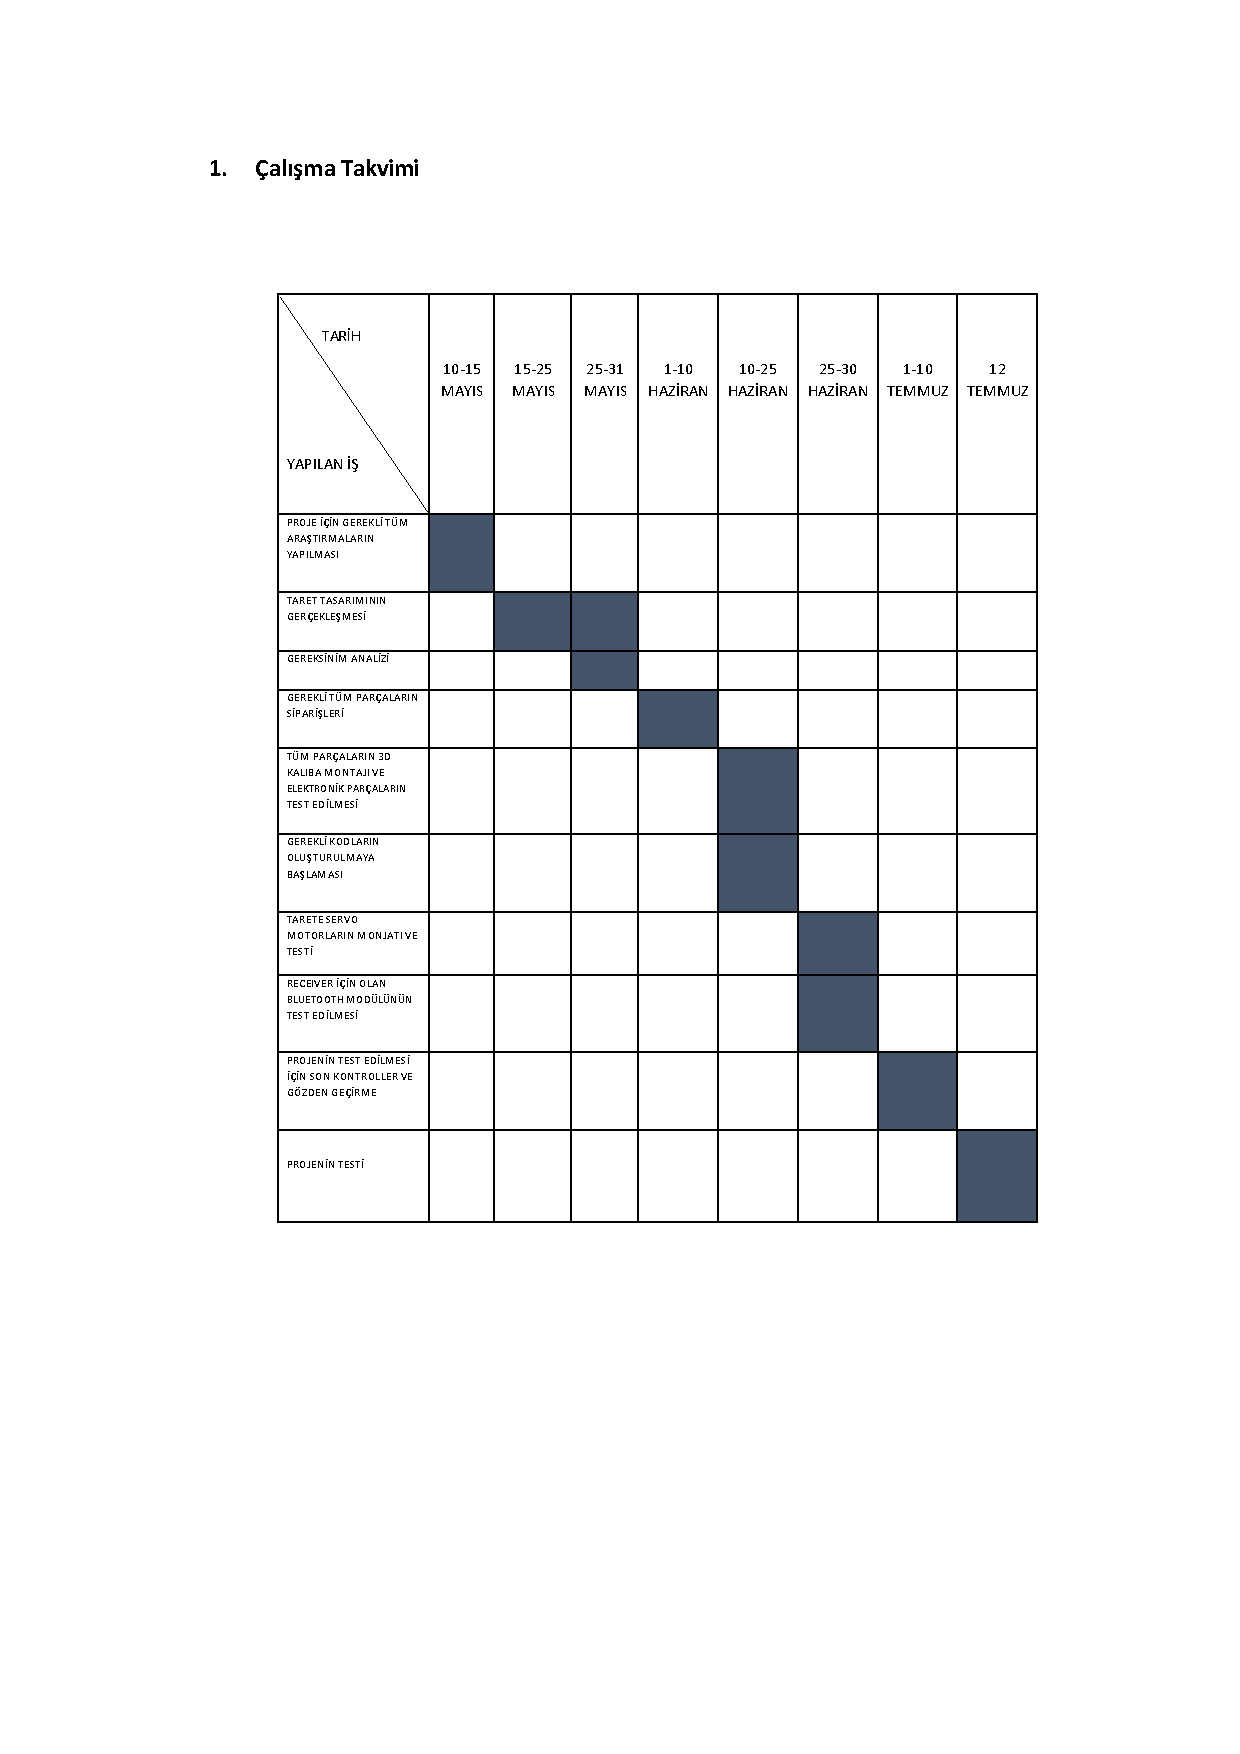
\includegraphics[width=148mm, height=225mm]{grafik/CalismaTakvimi.pdf}
   	\label{fig:CalismaTakvimiDM}
\end{figure}

\clearpage %ÇalışmaTakvimi
\chapter{A : ROBOT NEDİR?}
\label{BirinciBolum}

	Robotlar doğayı taklit eden insan hayatını kolaylaştıran makinelerdir. Robotlar, otonom ya da kumanda edilen, algılayıcıları, kontrol sistemi ve bedensel yapıları ile nesneleri tutmak, kavramak, hareket ettirmek, taşımak, üretim yapmak gibi amaçları yerine getirebilen elektronik, mekanik veya simetrik yapılardan oluşan yapay sistemlerdir.
    
    \clearpage
 
\clearpage
\section{A.1: Robotların Tarihsel Gelişimi}
\label{CH:AltBolum1.1}

	Robot kelimesi ilk olarak 1921 yılında sunulmuş olan bir tiyatro oyununda karşımıza çıkar. Ünlü Çek bilim kurgu yazarı Karel Capek tarafından yazılmış R.U.R. oyunu Çekoslavakya’ da sahnelenmiş bir bilim kurgu yapıtıdır. Yazar, kendi dili Çekce’ de işgücü anlamına gelen "robota" kelimesini oyunda kullanmış ve bu kelimenin lüteratürlere geçmesine yol açmıştır. KAYNAK [4]

\clearpage
\section{A.2: HABERLEŞME }
\label{CH:AltBolum1.2}

Haberleşme sistemleri temel olarak 3 elemandan oluşur:

• Verici

	Sistemdeki verici tarafından gönderilen bilgi alıcıya iletilmesinden önce iletilecek hale getirilir (yani veriye dönüştürülür), kendi güç kapasitesine göre iletim yaptığı mesafenin değişmesi süretiyle, gerekli kodlamaları yapar, hatta gerekirse kuvvetlendirme de yapılır.  
    
• İletim Ortamı 

	Sistemler arasındaki iletim ortamı verici tarafından sinyalin iletildiği ortama verilen isimdir. Bu iletim ortamları kablolu ve kablosuz olmak üzere ikiye ayrılır. Kablolu İletim Ortamının tanımını yaparsak; verilerin iletimi yanlızca bu kabloların bağlı olduğu modüller arasında gerçekleşir. Bakır, fiber optik, bükümlü, koaksiyel  kablolar vs. Kablosuz İletim Ortamının tanımı ise; bu ortamlarda iletişim, veriler en uygun alıcıyı kullanarak TV ve radyo yayınlarındaki gibi herkes tarafından alınabilmektedir. En verimli ortamları hava, su, boşluk vs. gibi doğal ortamlardır.  
    
• Alıcı 

	Vericide toplanan bilgi, bahsi geçen iletim ortamlarından geçtikten sonra alıcıya gelir. 

\clearpage
\section{A.3: Kablosuz İletişim }
\label{CH:AltBolum1.3}

Günümüzde kablolu haberleşmenin yanında kablosuz haberleşme de oldukça yaygınlaşmıştır. Bu kablosuz haberleşmeler kullanıcılara herhangi bir yerde herhangi bir anda iletişim kurma olanağı sağlıyor. Kablosuz haberleşme teknolojileri kablo kullanımını 5 kat azaltmaktadır. Bu sistem belli bir mesafede hareket özgürlüğü sağladığından sabit duran veya hareketli bir üründen bilgi almak/göndermek kablosuz haberleşme için büyük bir avantajdır. Tarihte ilk fikir, bilgisayar ve çevresindeki elektronik ürünlerin birbirleriyle kablosuz haberleşmesini sağlamaktı. Daha sonra bu düşünce genişledi ve daha da büyük alanlarda kullanılması hedeflendi. Dar alan kablosuz haberleşme sistemleri özellikle askeri alanda, tıpta, oto sanayide ve AVM'lerde kullanılmaya başlamakta ve gün geçtikçe kullanım alanları artmaktadır. Bu sistemdeki temel amaç, düşük güç harcayarak en az 10 metrelik bir alanda kablo olmaksızın güvenli bir haberleşme ağı kurmaktır. KAYNAK [2]

\clearpage
\section{A.4: Kablosuz Haberleşmenin Bazı Türleri}
\label{CH:AltBolum1.4}

	Bugüne dek birçok firma tarafından kablosuz haberleşme modellerini üretmek adına birkaç çeşit model üretilmiştir. 3G ve 4G, WI-MAX, Bluetooth ve WiFi gibi teknolojiler en popüler olanlarıdır. PAN’ ler için geçtiğimiz senelere kadar Bluetooth ve WiFi olmak üzere iki ana teknoloji bulunmaktaydı. Ancak her sistemin kolaylıkları ve yenilikleri olmasına rağmen bazı istekleri karşılayamazlar. PAN ağlarından biri olan ZigBee 1999 yılında FireFly çalışma grubu tarafından tasarlamaya başlamıştır. Bu sayede bazı istekler karşılanmıştır.

\clearpage
\section{A.5: Bluetooth (IEEE 802.15.1) }
\label{CH:AltBolum1.5}

	Bluetooth adını eski Danimarka Kralı Harald Blataad’ tan almıştır. Bluetooth genel olarak bina içi kablosuz ağ sistemi olarak tanımlanabilir. Tasarlanış amacı kısa mesafelerde düşük güç tüketmek suretiyle diğer komşu elektronik cihazlarla bağlantı kurarak veri alışverişinde bulunmaktır. Bluetooth birbirini kapsam alanında görme şartını ortadan kaldırmış olmasına rağmen güvenlik problemi ortaya çıkmış ve bu kamsam alanı içindeki sistemi haberleşecek olan sitemlerin girişim ve bayılmadan dolayı bağlantı kopma problemleri 6 oluşmuştur. Aynı zamanda Bluetooth sistemi kapsam alanı dışındaki sistemlerle de girişim oluşturabilmektedir.
\chapter{B: ARDUİNO}
\label{IkinciBolum}

	Arduino kullanımı ilk başta pek az kişi tarafından bilinmekteydi. kökenleri ise Wiring ve Processing projelerine dayanmaktadır. Henüz programlama deneyimi olmayan kişilere programlamayı öğretebilmek amacıyla processing programlama dili ve geliştirme ortamı oluşturulmuştur. 
    Teknik bilgisi az olan insanlara bilgi besleme adına da kolaylık sağlayan arduino, çevresiyle etkileşim içinde olan interaktif nesneler oluşturmak isteyen tasarımcılar için de büyük kolaylık sağlamaktadır.
    Arduino bir Giriş/Çıkış kartı ve Processing dilinin uygulamasını da dahilinde bulunduran bir fiziksel programlama platformudur. Arduino bilgisayar üzerinde çalışan yazılımlarda kullanıldığı gibi tek başına çalışan interaktif nesneler oluşturmak için de kullanılabilir.
    
	Arduino’ nun neden bu kadar çok tercih edildiğini maddeler halinde gösterirsek:  
    
\begin{itemize}
\item Windows, Linux, Mac gibi bütün platformlarda çalışabilen geliştirme ortamı ve sürücülerinin kurulumu çok kolay olmaktadır.  
\end{itemize}

\begin{itemize}
\item Zengin bir kütüphane barındırdığından Birçok karmaşık işleme kolaylık sağlayabilmektedir.
\end{itemize}
	
\begin{itemize}
\item İçerisinde aktarılan kodlar/programlar oldukça hızlı çalışmaktadır. 
\end{itemize}

\begin{itemize}
\item Başka donanımlarla da çalışabilmesi adına ek donanımlar içermektedir. Bu karta bağlanamayan sensör çeşidi yok desek yeridir.
\end{itemize}
    
\begin{itemize}
\item Benzer diğer devre kartlarına kıyasla fiyatı oldukça uygundur.
\end{itemize}
   
\begin{itemize}
\item Açık kaynak kodlu olması kullanmak isteyen herkesin özgürlüğine olanak sağlamaktadır. Misal bir eğitim kurumu Arduino için lisans parası ödemeden rahatça kullanabilir. KAYNAK [5],[6]
\end{itemize}


\clearpage 
\clearpage
\section{B.1: Arduino Çeşitleri: }
\label{CH:AltBolum2.1}

1. Arduino Uno 	

2. Arduino Nano	

3. Arduino Mega  

4. Arduino Mini ve Mini Pro 

5. Arduino Bluetooth 

6. Arduino Lilypad 20 	

7. Arduino Leonardo

8. Arduino Adk 		

9. Arduino Ethernet

\clearpage
\section{B.1.1: KULLANILAN MALZEMELER}
\label{CH:AltBolum2.2}

Arduino Nano 		x 1 --------------------------------------- 9v Pil				x 1

M2x10 Vida			 30 civarı	---------------------------------- M5x20 Vida x3

MG90s - Servo Motor	  x 3 ----------------------------- Makaron Kablo

HC-05 Bluetooth Modül 	x 1 -------------------------- LM2596 Voltaj Regülatörü x1

3D Printer Taret Kalıbı -------------------------------- Dirençler (10k, 330, 680) x3

FR207 Doğrultucu Diyot			x 1 -------------------------- Super Glue + Spray

Jumper Kablo --------------------------------------------- 2.1x5.5mm Jak Fişi x1

RFP30N06LE mosfet   x1 -------------------------------- Type 130 DC Motor x2

1.5mm Metal Çubuk x1 --------------------------------- Dupont Konnektörler

\begin{figure}[H]
	\centering
	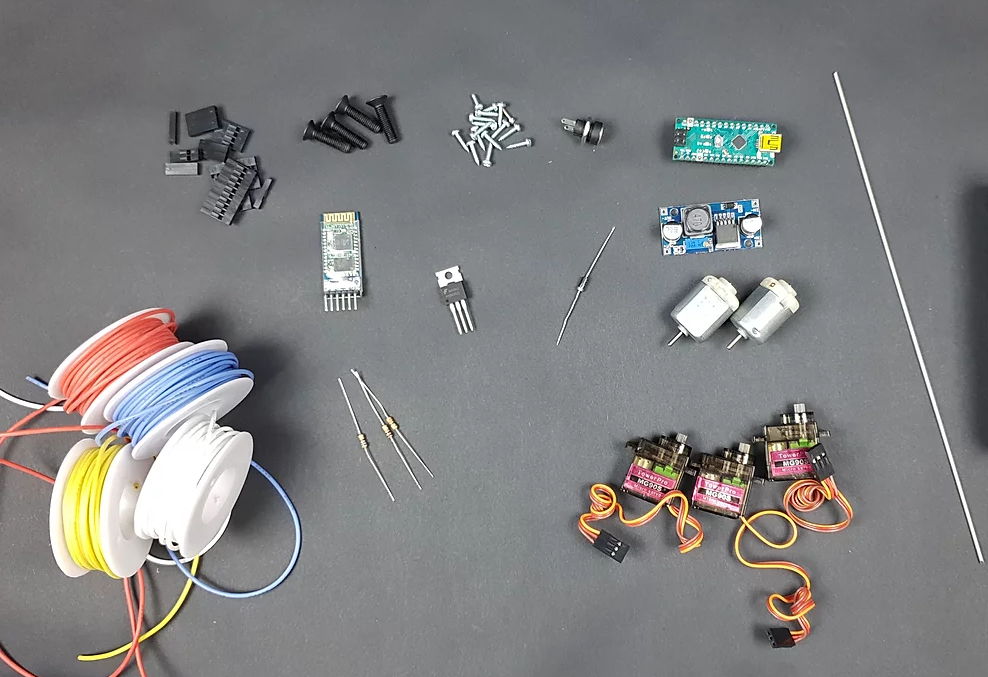
\includegraphics[width=150mm]{grafik/Malzemeler.png}
    \caption{Not: Projede Kullacağım Malzemeler (Bazı parçaları eksik ve 3D kalıp hariç görüntüsüdür.)}
	\label{fig:MalzemelerDM}
\end{figure}



\clearpage
B.2: Arduino Uno 
\label{UcuncuBolum}


	Geliştirilen birçok projede kullanılan en popüler devre kartıdır. Üzerinde birkaç donanım barındırmaktadır. Bunlar: Atmega328 mikrodenetleyici, 16 MHz kristal, güç regülatörü, USB bağlantı portu, gibi bileşenler bulunuyor. Üzerindeki USB dönüştürücü sayesinde hem gerekli kodlar aktarılabilmekte hem de bilgisayar ile iletişim kurulabilmektedir. Kart, üzerindeki fiş jakı sayesinde adaptör tarafından veya üzerindeki USB portu sayesinde kurulan USB bağlantısı tarafından beslenebilmektedir. Arduino Uno kartının ön ve arka görünümü sırasıyla, Şekil 2 ve Şekil 3'de gösterilmiştir.

\begin{figure}[H]
	\centering
	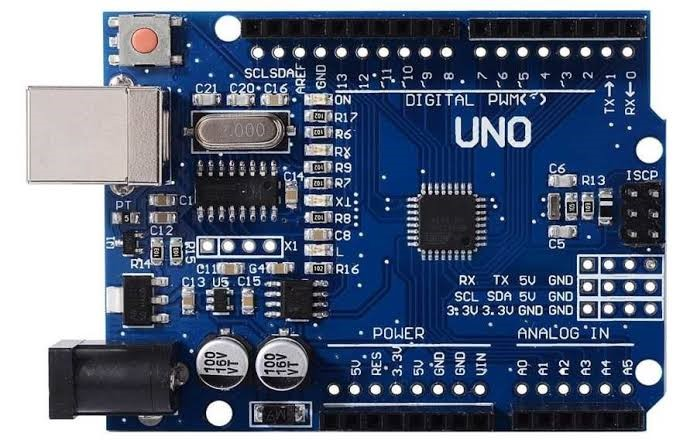
\includegraphics[width=80mm]{grafik/ArduinoOnden.jpg}
    \caption{Arduino Uno (Klon) kartının ön görünümü}
	\label{fig:ArduinoOndenDM}
\end{figure}
\begin{figure}[H]
	\centering
	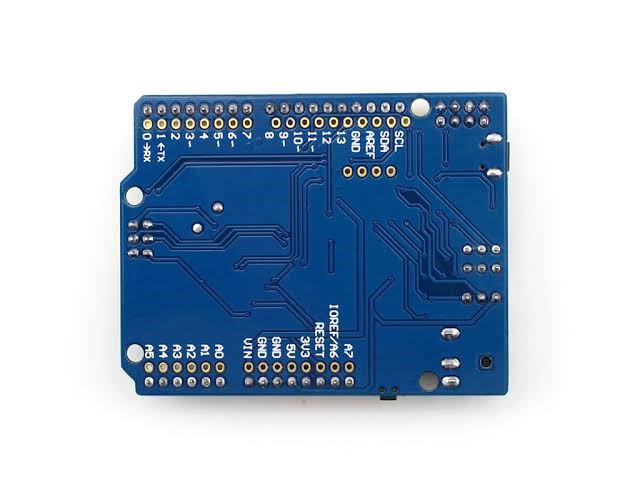
\includegraphics[width=100mm]{grafik/ArduinoArkadan.jpg}
    \caption{Arduino Uno (Klon) kartının arka görünümü}
	\label{fig:ArduinoArkadanDM}
\end{figure}

\clearpage 
B.3: Servo Motor
\label{DorduncuBolum}

	Servo motorlar çoğu projenin hareketini sağlamakta ve olmazsa olmazlardandır. CNC'lerde, model uçaklarda, RC arabalarda, 3D Printerlarda ve küçük güçteki birçok robot uygulamalarında kullanılmaktadır. Servo motor içerisinde geri besleme potansiyometresi, DC elektrik motoru, DC motor konum kumanda elektroniği ve planetar dişli sistemi bulunmaktadır. Bu motorlar projemde tasarlanan taretin gövde, baş ve tetikleme hareketlerini gerçekleştirmek amacıyla kullanılacaktır. Servo motorun blok diyagramı, projede kullanılan modeli ve devre şeması sırasıyla, Şekil 4, Şekil 5 ve Şekil 6’da gösterilmiştir.

\begin{figure}[H]
	\centering
	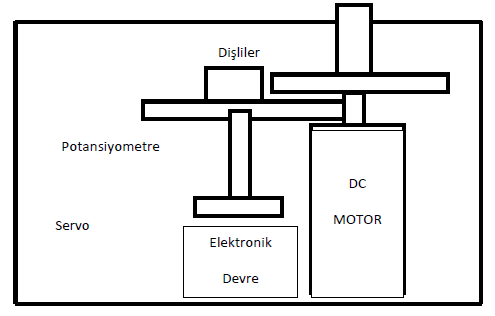
\includegraphics[width=60mm]{grafik/MG90s-Diyagram.png}
    \caption{Servo motorların genel iç blok diyagramı}
	\label{fig:MG90s-DiyagramDM}
\end{figure}
\begin{figure}[H]
	\centering
	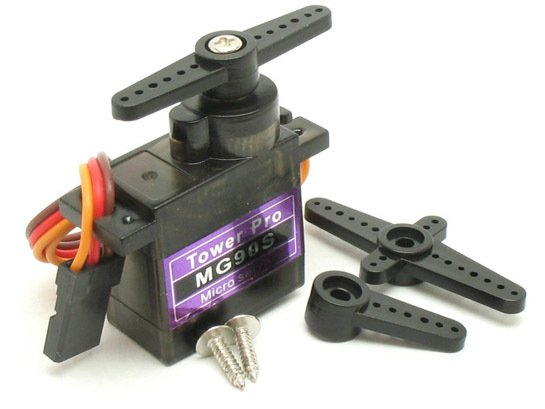
\includegraphics[width=60mm]{grafik/MG90s.jpg}
    \caption{Projede Kullanılan MG90s Servo}
	\label{fig:MG90sDM}
\end{figure}
\begin{figure}[H]
	\centering
	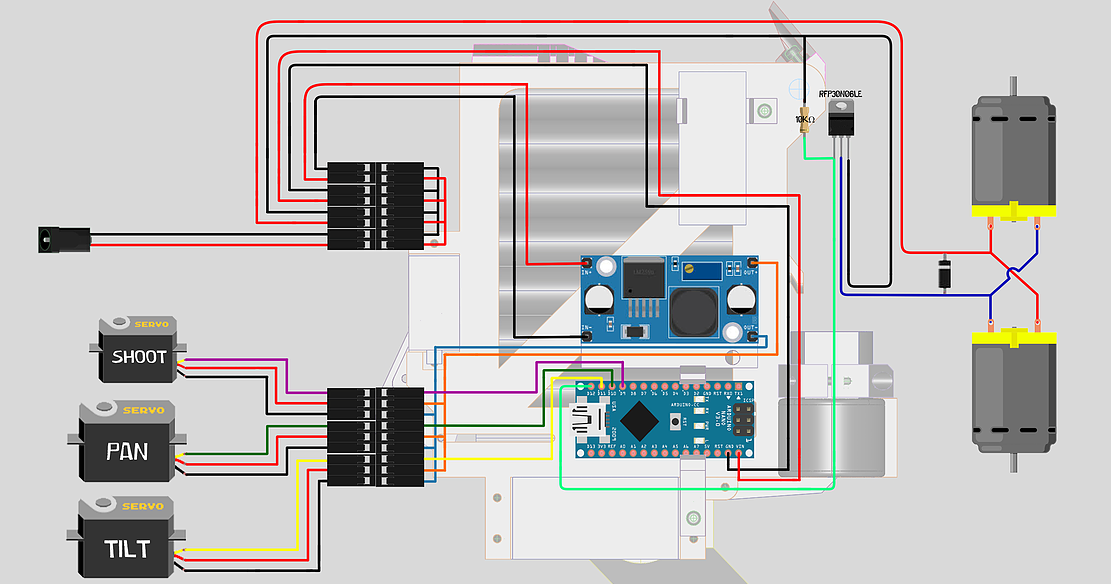
\includegraphics[width=70mm]{grafik/MG90s-Devre.png}
    \caption{Servo Motorların Projedeki Devre Şeması}
	\label{fig:MG90s-DevreDM}
\end{figure}

\clearpage 
\textbf{B.3.1: TEKNİK ÖZELLİKLER:}
\label{CH:AltBolum4.1}

MG90s Servo Motor Özellikleri:

•	Çalışma tork: 2 kg/cm

•	Hızı: 0.11 sn/60° (4.8 V)

•	Çalışma aralğığı: 4.8 - 6.0 V

•	Çalışma sıcaklığı: 0°-55°

•	Ölü bant ayarı: 5 mikrosaniye

•	Dönme açısı: 180 derece

•	Çalışma gerilimi: 4.8 V - 6.0 VDC

•	Yapısal Malzeme: bakır metal diş, çekirdeksiz motor, çift bilyalı rulman

•	Boyutu: 23 x 12x 29 mm


\clearpage
\textbf{B.4: HC-05 Bluetooth Modül}
\label{YedinciBolum}

	HC-05 Bluetooth modülü,  kablosuz seri haberleşme projeleri için yapılmıştır. Bu modül bluetooth 2.0’ı destekleyen, 2.4GHz frekansında haberleşme yapılmasını sağlar. Haberleşme esnasında açık alanda yaklaşık 10 metre haberleşme mesafesine sahiptir. Modülün haberleşme bağlantısı serial yani UART olduğundan kolay ve hızlı bir kullanımı vardır. Üzerinde bulunan RX ve TX pinleri sayesinde iletişim sağlanır. Bu pinler kullanılacak olan devre kartınının sırasıyla TX ve RX pinlerine bağlanır. Ayrıca bu pinler yardımıyla AT komutlarını kullanarak modülün isim, şifre,baud rate değeri, gibi çeşitli özellikleri değiştirebilir. KAYNAK [3]
    
	Projede ise bu modül kablosuz haberleşme için kullanılmaktadır. Bilgisayar veya mobil üzerinden alınan analog veriler bu modül sayesinde tarete aktarılmaktadır. Bu sayede kullanıcı tarafından yapılan hareketleri anlık olarak taret üzerinde de gözlemleyebiliriz. Bluetooth modül Şekil 7de gösterilmiştir.

\begin{figure}[H]
	\centering
	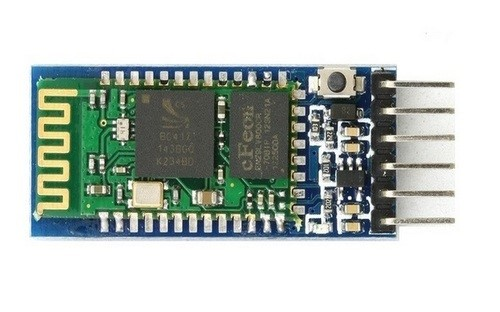
\includegraphics[width=100mm]{grafik/Bluetooth.jpg}
    \caption{Projede Kullanılan HC-05 Bluetooth Modülü}
	\label{fig:BluetoothDM}
\end{figure}

\textbf{Dikkat:} HC-05 Bluetooth modülü devre kartındaki 3.3V pinine bağlantı yapılarak veya uçları arasında dirençler bağlayarak çalıştırılması gerekmektedir. HC-06 Bluetooth modülü ise 5V pinine bağlantı yapılarak veya yine direnç bağlanarak çalıştırılmalıdır.

\textbf{Bilgi:} Kodları hatasız bir şekilde Arduino’ya aktarabilmek için Arduino üzerindeki RX ve TX pinlerine bağlı kabloları aktarma işleminden önce sökmek gerekiyor. Bu işlem yapılmazsa kod aktarımı sırasında portların meşgul olduğuna dair hata alabiliriz. 

\clearpage 
\textbf{B.4.1: TEKNİK ÖZELLİKLER:}
\label{CH:AltBolum7.1}

•	Çalışma Gerilimi: 3.3 V - 5 V,

•	Akım: 50 mA,

•	Bluetooth Protokolü: Bluetooth 2.0+EDR,

•	Haberleşme frekansı 2.4GHz,

•	Hassasiyet: ≤-80 dBm,

•	Çıkış Gücü: ≤+4 dBm,

•	Asenkron Hız: 2.1 MBps/160 KBps,

•	Senkron Hız: 1 MBps/1 MBps,

•	Güvenlik: Kimlik Doğrulama ve Şifreleme,

•	Boyutları: 43 x 16 x 7mm,

HC-05 Modülünün devre şeması Şekil 8’de gösterilmiştir.

\begin{figure}[H]
	\centering
	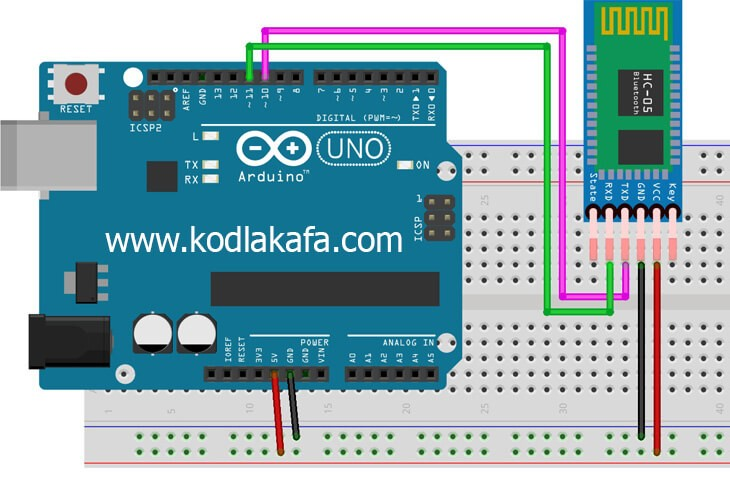
\includegraphics[width=120mm]{grafik/BluetoothFritzing.jpg}
    \caption{HC-05 Modülünün Bağlanma Şekli (Fritzing)}
	\label{fig:BluetoothFritzingDM}
\end{figure}

\clearpage
 
\textbf{B.5: 3D Taret Modeli}
\label{SekizinciBolum}

Taretin baskısı 3D yazıcılar vasıtasıyla PLA+  Filament kullanılarak yapıldı. Kendi oluşturmuş olduğum 3D modelleri ile Github üzerindeki üyerlerin modellerini mix ederek aşağıdaki modelleri elde etmiş oldum. 3D modeli oluşturmak için Blender programını kullandım. Taretin 3D modelleri Şekil 9’da gösterilmiştir. KAYNAK [1]

\begin{figure}[H]
	\centering
	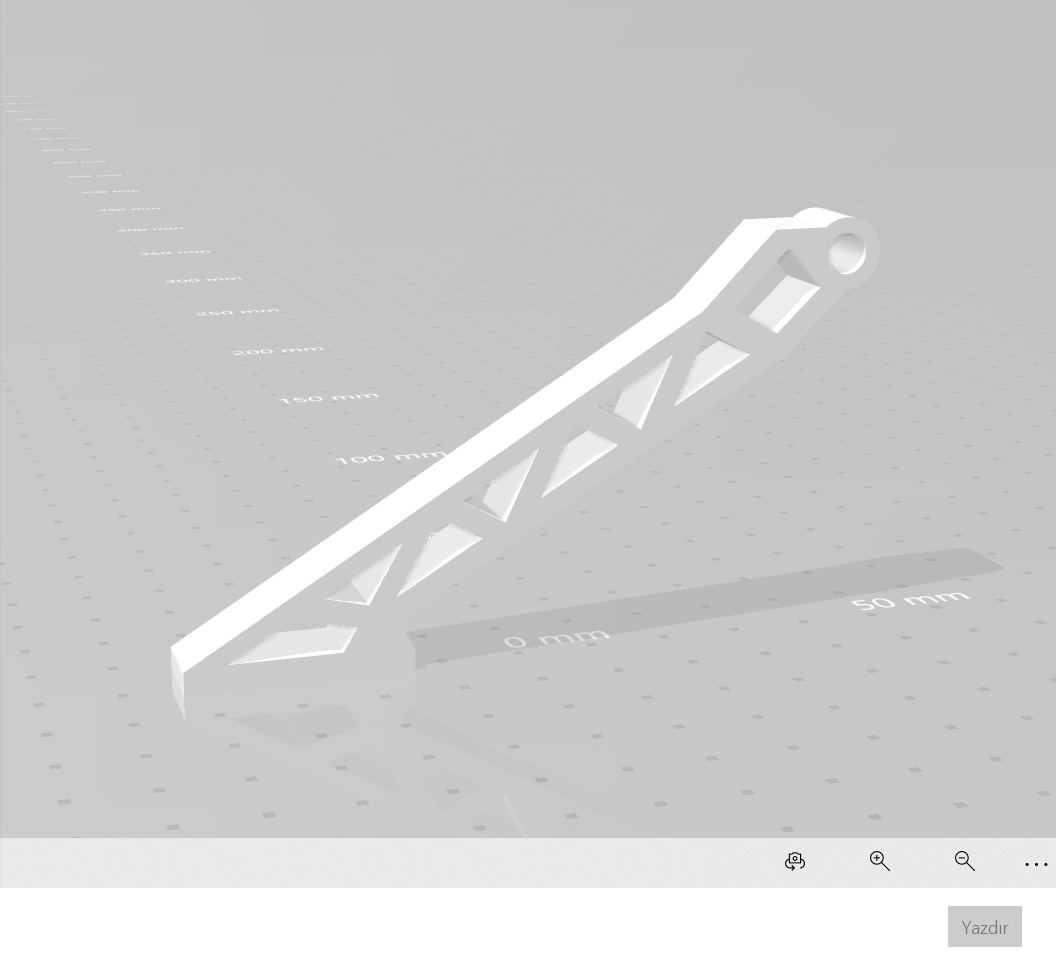
\includegraphics[width=50mm]{grafik/3D_Bacak.png}
    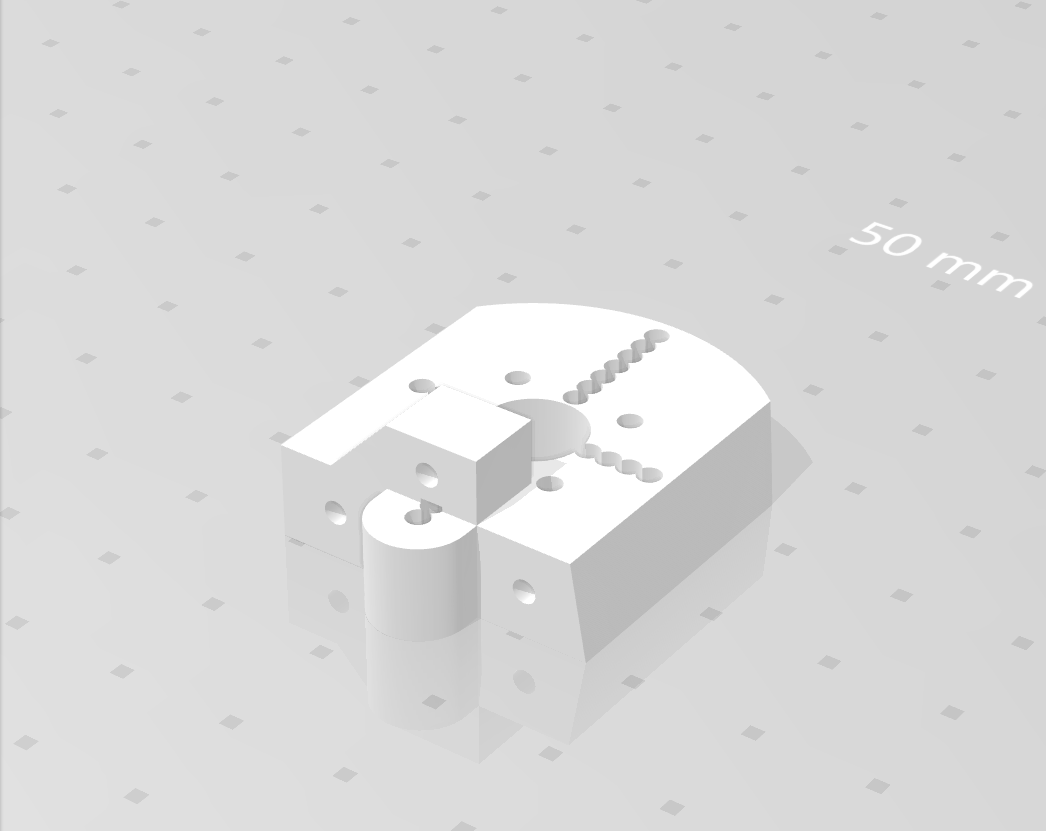
\includegraphics[width=50mm]{grafik/3D_EgilimAltDestegi.png}
    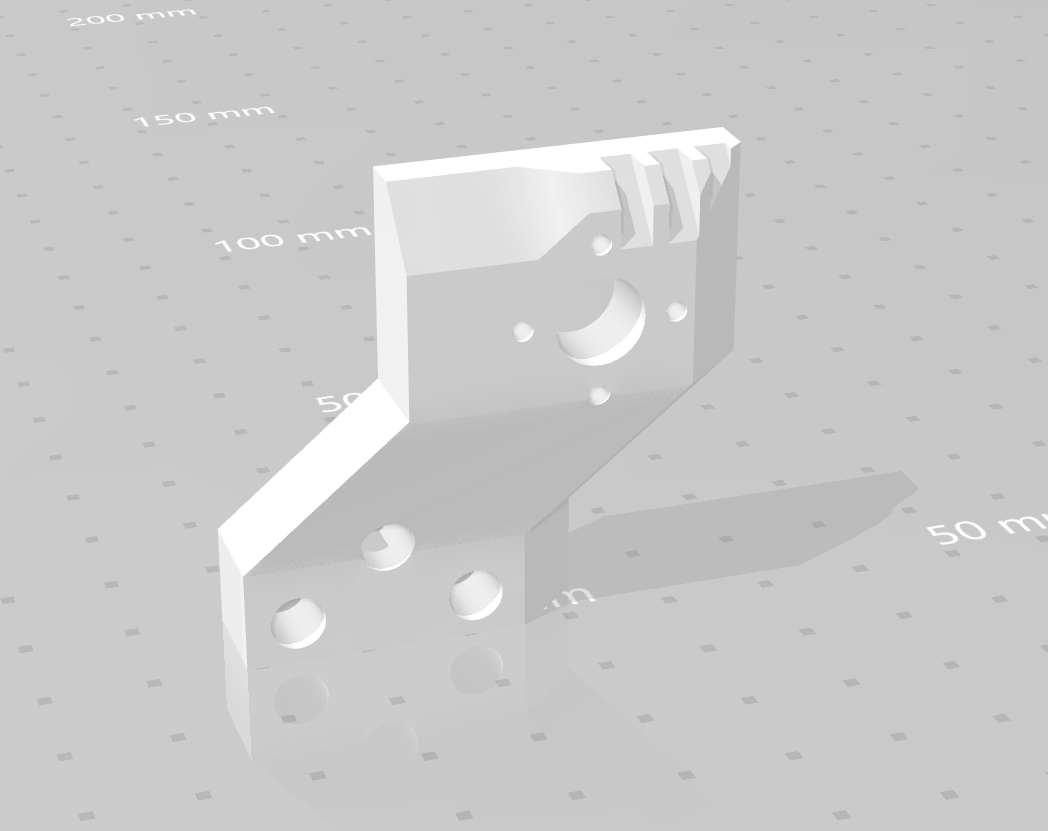
\includegraphics[width=50mm]{grafik/3D_EgilimUstDestegi.png}
    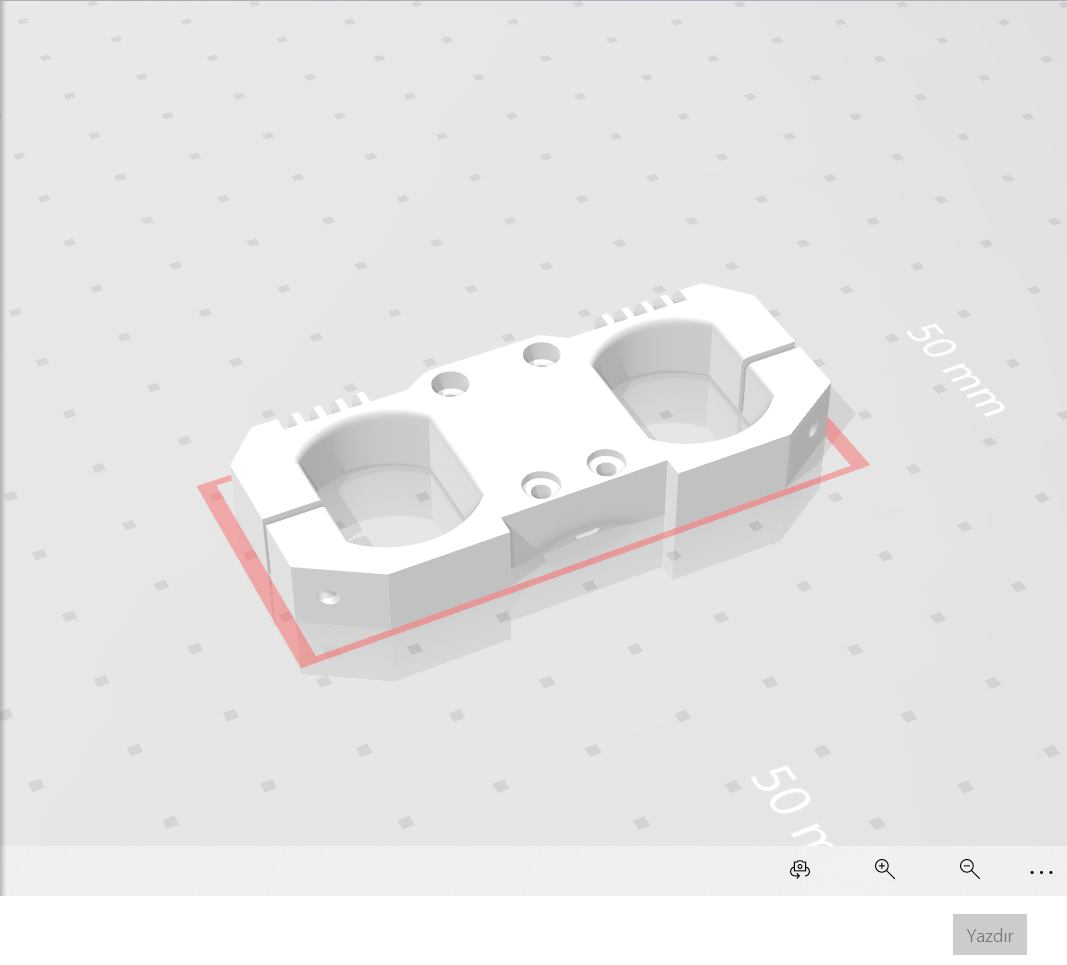
\includegraphics[width=50mm]{grafik/3D_MotorDestek.png}
    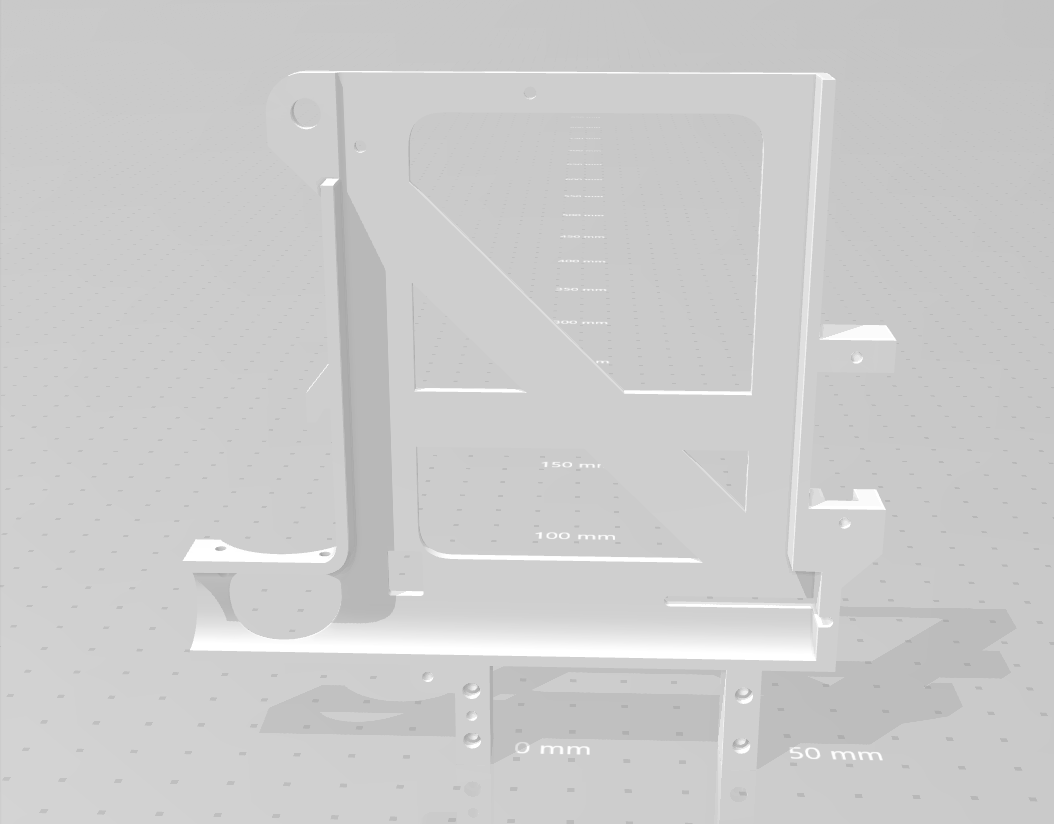
\includegraphics[width=50mm]{grafik/3D_NamluPlatformu.png}
    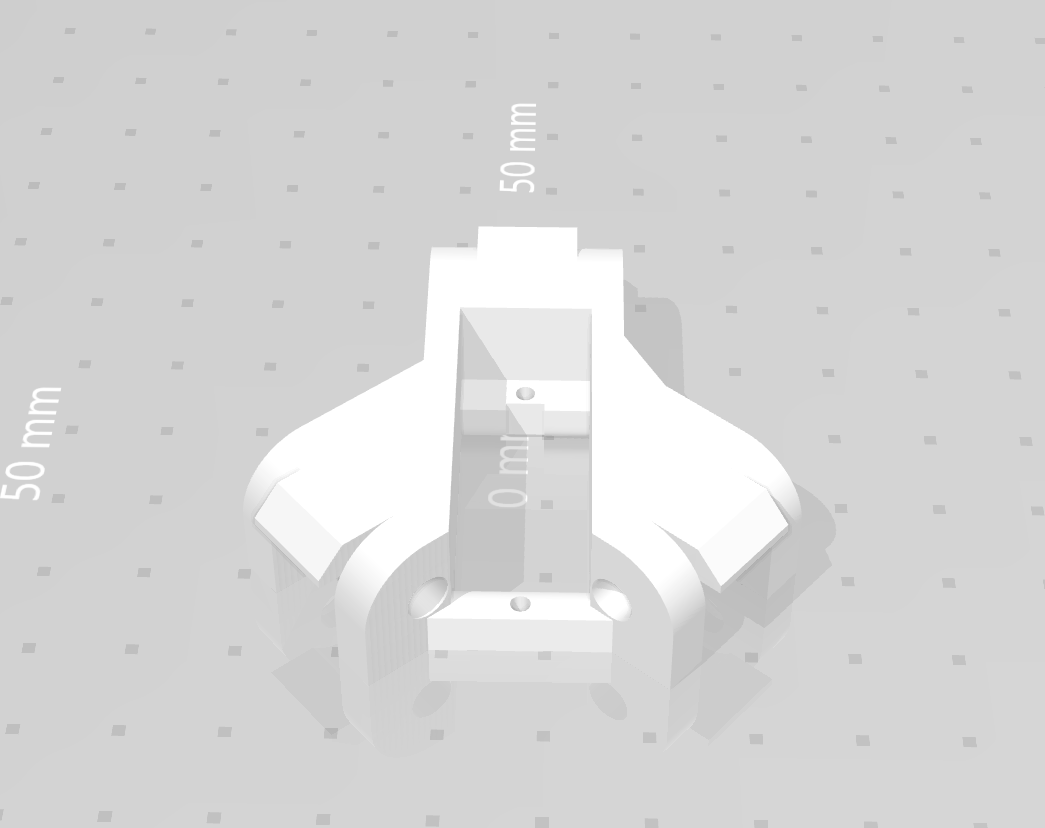
\includegraphics[width=50mm]{grafik/3D_Temel.png}
    
    \caption{Taret 3D Model Örnekleri}
    \label{fig:Taret1,2,3,4,5,6DM}
\end{figure}

\clearpage 
\textbf{C: Programlama Aşaması }
\label{DokuzuncuBolum}

Tüm devrelerin montajı tamamlandı ve projenin programlama aşamasına geçildi. Bu aşamada ilk önce fare hareketlerinin analog değerleri serial monitörden okunarak hassasiyet değerlendirmesi maksatıyla tam değerleri bulundu. Arduino NANO devre kartı ise okunan değerleri projede kullanılan servo motorlara dikey ve yatay açısal bilgileri gönderecek şekilde programlandı. Tüm kodlamalar Arduino IDE programı vasıtasıyla Bilgisayardan USB kablo ile Arduino NANO Mikrodenetleyicisine aktarıldı.

\begin{figure}[H]
	\centering
	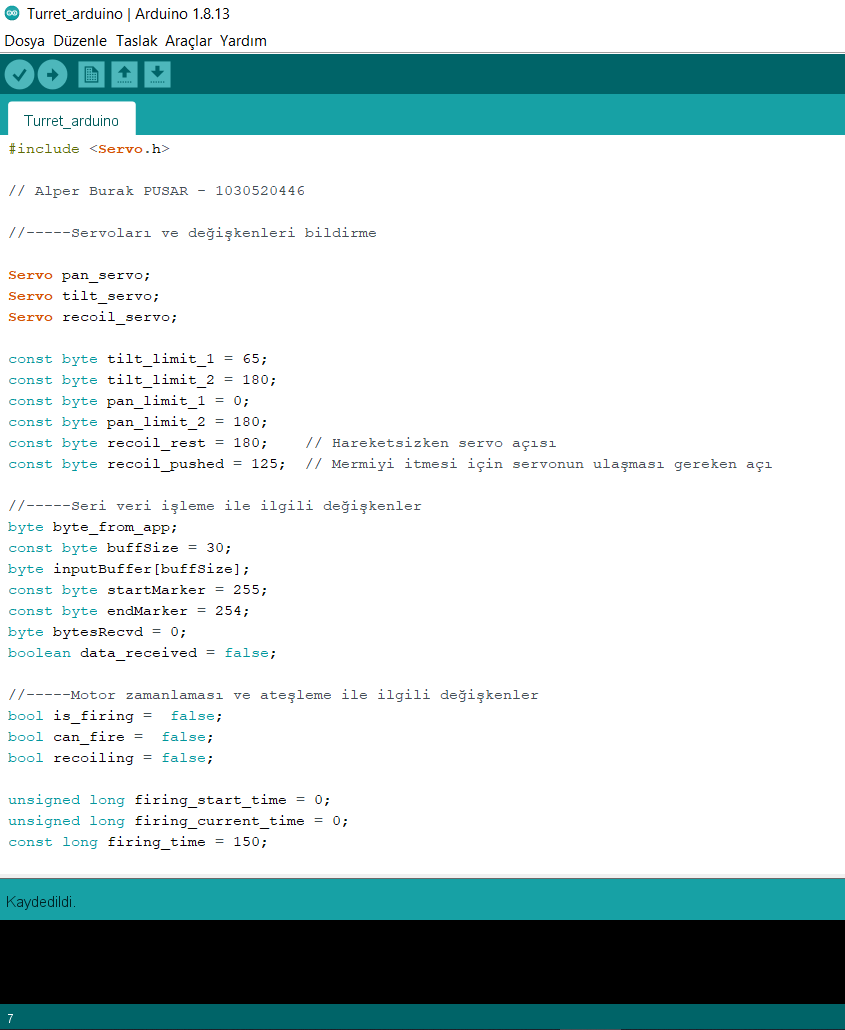
\includegraphics[width=120mm]{grafik/Kod 1.png}
	\label{fig:KodDM}
\end{figure}
\begin{figure}[H]
	\centering
	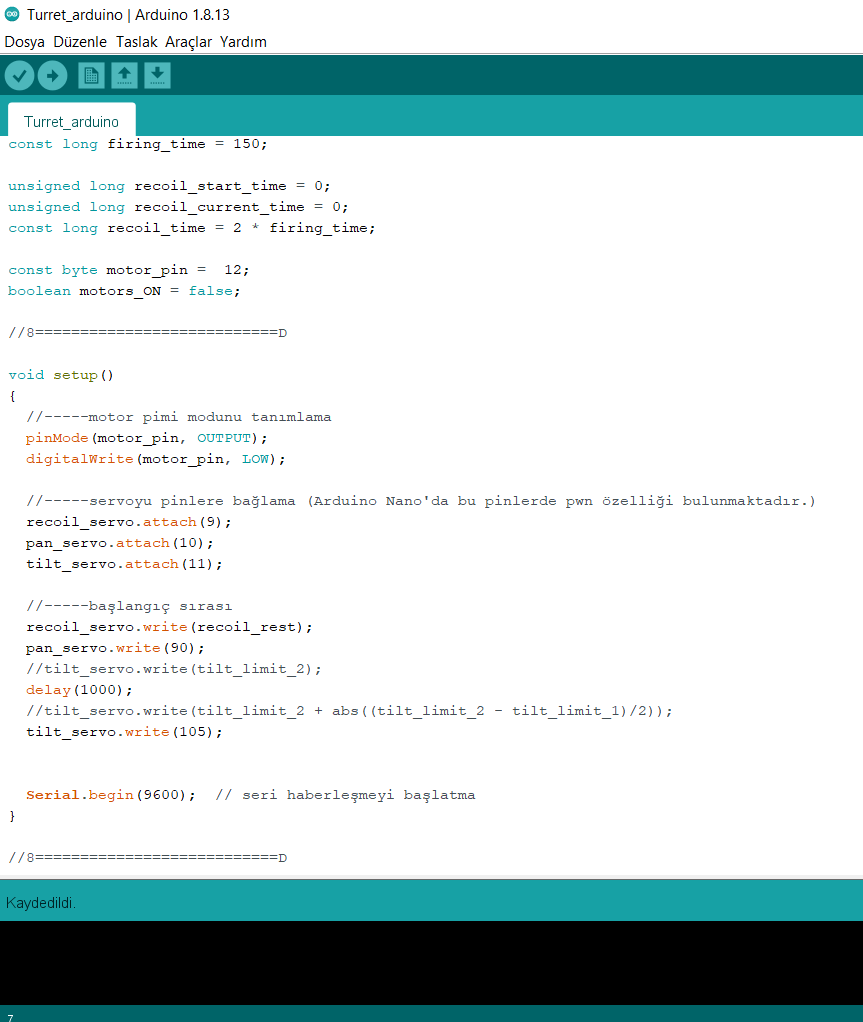
\includegraphics[width=120mm]{grafik/Kod 2.png}
	\label{fig:KodDM}
\end{figure}
\begin{figure}[H]
	\centering
	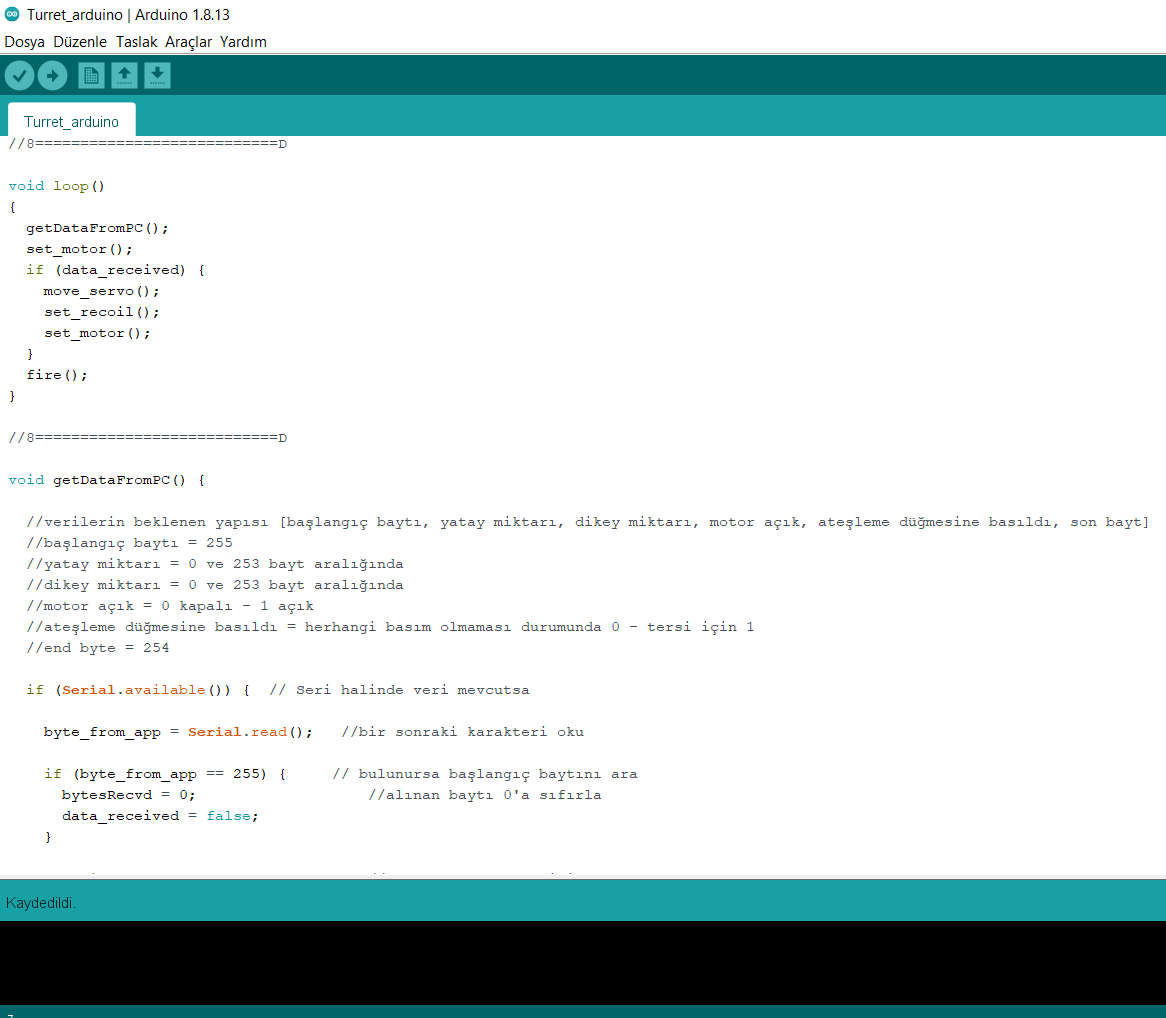
\includegraphics[width=120mm]{grafik/Kod 3.png}
	\label{fig:KodDM}
\end{figure}
\begin{figure}[H]
	\centering
	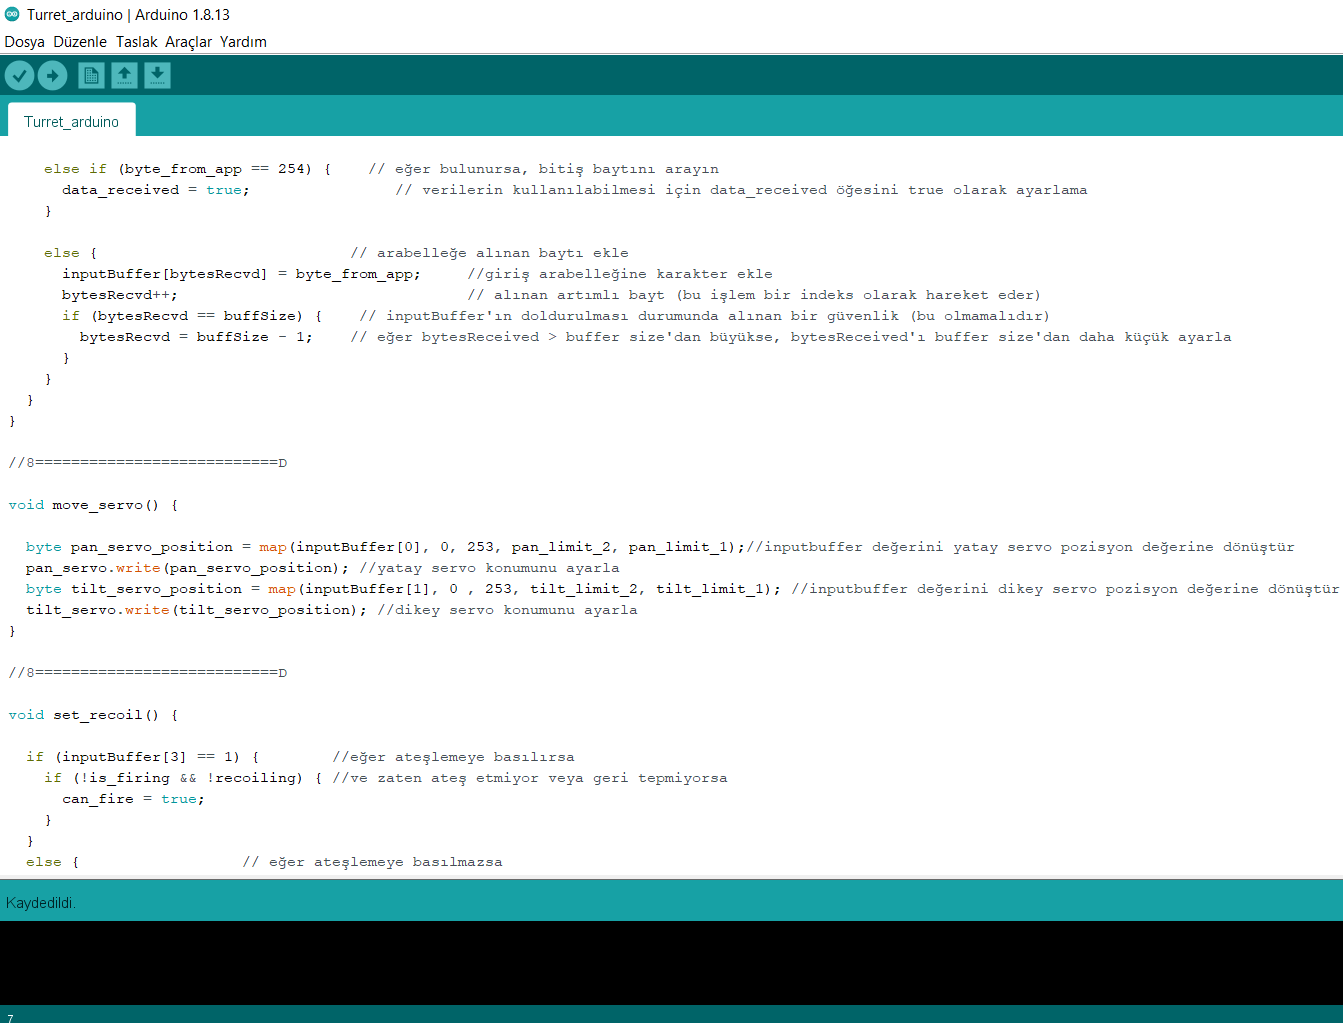
\includegraphics[width=120mm]{grafik/Kod 4.png}
	\label{fig:KodDM}
\end{figure}
\begin{figure}[H]
	\centering
	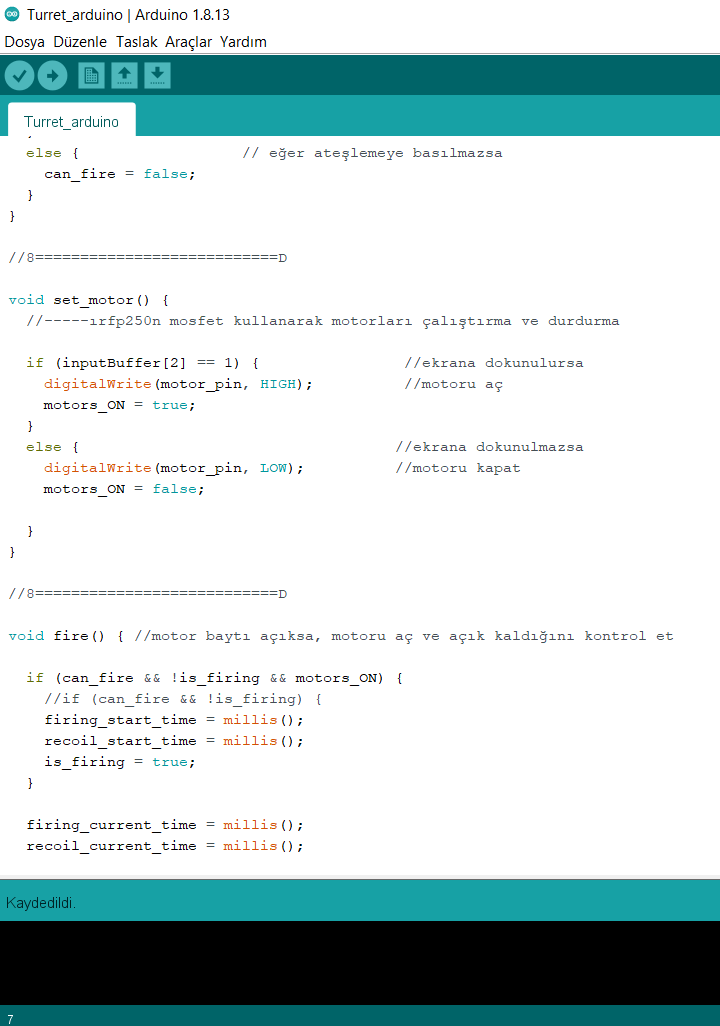
\includegraphics[width=120mm]{grafik/Kod 5.png}
	\label{fig:KodDM}
\end{figure}
\begin{figure}[H]
	\centering
	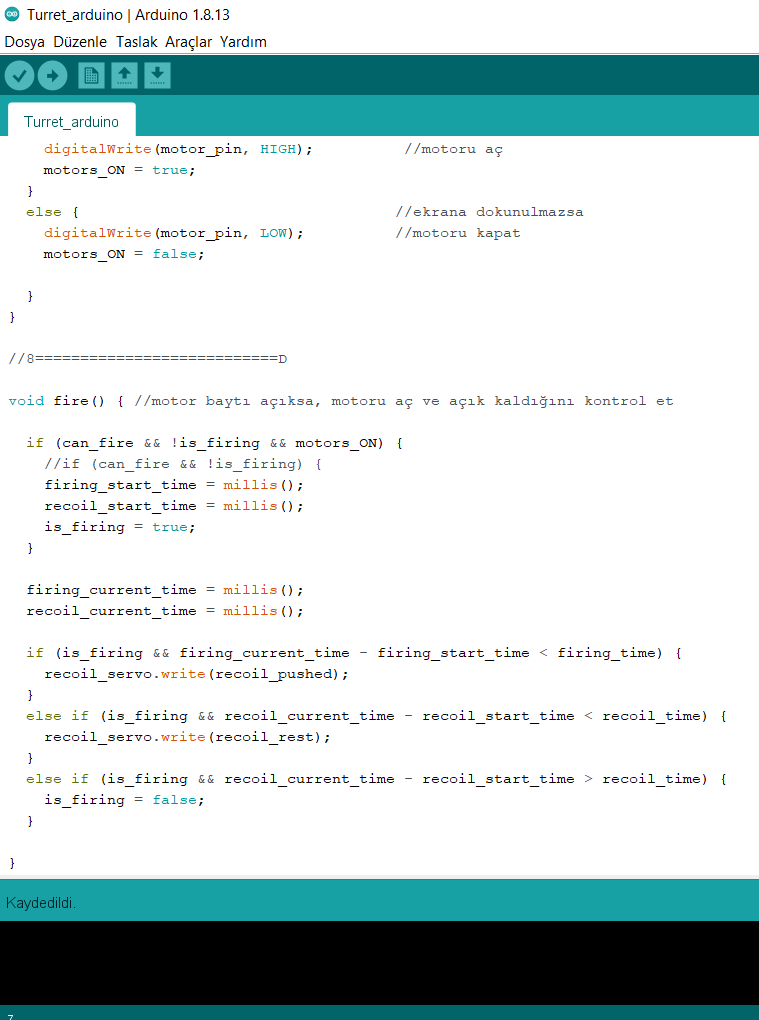
\includegraphics[width=120mm]{grafik/Kod 6.png}
	\label{fig:KodDM}
\end{figure}

\clearpage  
\textbf{D: SONUÇLAR }
\label{BolumSonuc}

	Yazılım ve Elektronik alanlarında yapılan yeni projeler ve devam eden çalışmaların en önemlileri insan sağlığını koruyacak türde veya global teknolojiye ayak uydurarak askeri ya da endüstriyel alanlarda gelişime açık olanlarıdır. Bu fikirle başladığım projeyi tamamlamak için amaçladığım gibi tareti kontol eden kişinin verdiği komutları veri kaybı olmadan tarete ulaşmasını sağlayabilmek vasıtasıyla tasarlanan taretin hedefe isabetli atışlarını gerçekleştirdim. Bu işlemin kullanıcı ve taret arasında kablosuz haberleşme ile sağlandığını vurgulamak gerekir.
    
Bu projeyi gerçekleştime aşamalarında birçok sıkıntıyla karşılaştım. İlk karşılaştığım sıkıntı satın almış olduğum arduino nano kartında arıza olmasıydı. Bu kartın hatalı olduğunu anlatıktan sonra yenisi temin ettim. ancak bu bozuk kartla işlem yapmaya kalkarken sanırsam hc-05 bluetooth modülümün de hasar aldığını farkettim ve onu da değiştirmek zorunda kaldım. Projede kullanılmasını uygun gördüğim FR207 hızlı diyot ve rfp30n06le mosfeti birçok yerde aradım ancak bulamadım. diyotun özellikleri 2A 100V değerlerini gösterirken mosfet ise 30A 60V değerlerini göstermekte. Ancak değindiğim gibi bu modülleri temin edemedeğimden bunların yerine BY298 hızlı diyot (2A 400V) ve ırfp250n mosfet (30A, 200V) modüllerini kullanmaya karar verdim. Bu modüller DC motorlara bağlantı kurduğundan, muhtemelen bu karar değişimden dolayı proje testi esnasında asıl büyük sıkıntıyı burada yaşadım. DC motorların güç kaçağı veya geri besleme gibi sıkıntılardan olsa gerek devreyi stabil tutamadım. bu kısım beni gerçekten çok uğraştırdı. İlk başlarda sıkıntının ne olduğunu da tam anlayamadım. En sonunda Voltaj dengesini sağlayarak devreyi stabil tutabildim.

Projenin sunumunu ayrı şekilde temin edeceğimden bu final tezine ekleme yapabileceğim kodlama, sonuç ve yorumlamalardan başka birşey kalmıyor. Zaten projenin son halini yazımdan çok videodaki anlatıma döktüm. Eminim yeterli gelecektir.

\clearpage 
\textbf{E: YORUMLAR VE DEĞERLENDİRME }
\label{BolumSonuc}

	Bu tarz robotik projeleri yapmaktan gerçekten keyif alıyorum ve kendimi bu alana yönelik geliştirmek istiyorum. Yaptığım proje ve bundan öncekilerin de bana katkısının büyük olduğunu düşünüyorum. Başlarda elektronik komponentler ve devre kartları üzerine pek bilgim yoktu ancak şuan bu tarz projeleri bitirmemin, bunları özellikle de tek başıma yapmanın bana katkısı büyük oluyor. Tüm araştırmalar ve analizler bana kalıyor ve bu sayede bilgi edinme hızım gayet hızlı ilerliyor. Ülkemizde hala gelişmekte olan robotik alan projeleri yurtdışında bazı bölgelerde fazlasıyla gelişmiş durumda ve imkanım olursa kenidimi bu firmalarda görmeyi isterim. Bunu da hedeflemek adına kendi gelişimimi bu karara göre yönlendireceğim.

\clearpage 
\textbf{KAYNAKLAR}
\label{CH:BolumKaynakca}

[1]. Github Users, Multi persons, Arduino Turret, Available: https://github.com/

[2]. The Extendedsystem website. Available: http://www.extendedsystems.com/

[3]. Haartsen, J. C., The Bluetooth Radio System, IEEE Personal Communications 

[4]. Çamoğlu, D., Kontrollü Robotik, Dikeyeksen Yayıncılık, Şubat 2011. 

[5]. Taşdemir, C., Arduino, Dikeyeksen Yayın Dağıtım, Yazılım ve Eğitim Hizmetleri San. ve Tic. Ltd. Şti., İstanbul, 2012. 

[6]. D. İbrahim, PIC Mikrokontrolör Robot Projeleri, Bileşim Yayıncılık Fuarcılık ve Tanıtım Hizmetleri A.Ş., İstanbul, Türkiye, 2005.

\clearpage 

\bibliographystyle{erciyesfbe} %% References style filename 
%\bibliography{referanslar}	 
%\appendix
%\input{ek2.tex}

\textbf{EK 3. Standartlar ve Kısıtlar Formu}
\label{CH:BolumEkler3}

\begin{figure}[H]
	
\includegraphics[scale=1.3]{grafik/eru.jpg}
    \label{fig:EruLogoDM} \centering Erciyes Üniversitesi Mühendislik Fakültesi Bilgisayar Mühendisliği
\end{figure} 

\textbf{STANDARTLAR VE KISITLAR FORMU}
\\ \hline 

\textbf{1. Projenizin tasarım boyutu nedir?}

 	Plastik mermi kullanacak şekilde Minimizal bir boyutta olup ergonomik olması hedeflenmektedir. Kullanımı ve gerçekleştirilmesi karmaşık olmayacak. Savunma sanayide kullanılabilir olup, birçok askeri ve manevi ihtiyacı karşılayacaktır.
    
\textbf{2. Üniversite eğitim süreci boyunca girdiğiniz derslerden edindiğiniz hangi deneyim ve bilgileri kullandınız?}

	Temel olarak Arduino programını kullanmamıza olanak sağlayan elektronik derslerinden ve gömülü sistemlerden projenin devresini oluşturmakta zorluk çekmedim. Ayrıca mikroişlemciler dersini almamın bana bu proje üzerinde araştırma kolaylığı sağladığı da aşikardır.
    
\textbf{3. Projenizde bir mühendislik sorununu kendi yöntemlerinizle formüle edip, çözüm sağladınız mı? }

	Yorumlama ve Değerlendirme kısmında bahsettiğim gibi bu kısım hakkında şuan için verebileceğim bir bilgi yok.
    
\textbf{4. Dikkate aldığınız esas kısıtlar nelerdir? }

a) Teknoloji

	Sürekli gelişen teknolojiye her zaman güncel kalmak kimseyi geride bırakmaz. Bu izlenimle projenin mevcut teknolojiye ayak uydurması ve başka projelere de ilham kaynağı olması hedeflenmektedir. Her yeni çıkan teknolojiler izlenmeli ve mümkün olan en yeni parçalarla ürünü sunmak gerekmektedir.
    
 b) Ekonomi
 
	Projenin üretim maliyeti, projenin hayata geçmesi ve zarar edilmemesi açısından oldukça önemli bir faktördür. Projede kullanılacak olan parçaların performansı ve fiyatı incelenerek fiyat/performans oranları çıkarılmaya çalışılmıştır. 


c) Çevre sorunları: 

	Proje düşük enerji tüketimi ile çevre dostu olduğundan ve çevreye verebileceği herhangi bir zararı bulunmadığı için oldukça kullanışlıdır.
    
d) Üretilebilirlik: 

	Projede kullanılan malzemelerin satış fiyatları oldukça uygundur. Böylelikle bu çaplı minimizal (aynı zamanda deneysel) bir projenin hayata geçirilmesi için büyük bir imkân sağlanıyor. Projeyi dinamik ve performanslı hale getirerek endüstriyel anlamda seri üretime geçilme imkânı sağlanmalıdır. Şuanda da birkaç benzer örneği mevcuttur.
    
e) Sürdürülebilirlik:

	Günümüz çağında Mikrodenetleyici kontrollü kablosuz sistemler, yeni gelişmekte olan bir sektördür. Mikroişlemcilerin, entegre parçaların, transistörlerin ve sensörlerin gelişmesiyle ilerde çok daha gelişeceğini tahmin etmek zor olmasa gerek. Proje kolay geliştirilebilir olduğundan bu imkana olanak sağlıyor. Ayrıca farklı proje ve sistemlerle ortak noktalarda birleştirilebilecek bir projedir. 
    
f) Sağlık: 

	Robot elin üretimi için kullanılacak olan PLA+ Filamentin bileşenleri mısır besi dokusundan elde edilen nişasta ve şeker pancarı gibi bitkisel, yenilebilen ürünlerden elde edilir. Bu nedenle doğaya hiçbir şekilde zarar vermez. Isı ile oluşabilecek sağlığa zararlı ve kötü koku salınımı yapan gazlar ortaya çıkarmaz.
    
 g) Güvenlik: 
 
	Projenin devresindeki tüm bileşenler voltaj regülatörü + trimpot ile dengelenmiş olup 5V ile çalışmaktadır ve hiçbir şekilde güvenlik açığı teşkil etmezler.

\clearpage 

\end{document}
